
\subsection{Sustained CW-NIR stimulation protocol}
\label{sect:sustained-protocol}
After the isolation of the \textit{Lymnaea stagnalis} neural system, we searched for suitable neurons in the right parietal ganglion, i.e., cells with spontaneous activity preferably with fast activity and shoulder or symmetrical type in the spike waveform. 
Once the target neuron was identified, the laser was set-up. A lens with focal distance of $f$=50mm was used and no polarizer was installed on the optical path. Guided with the microscope camera, the laser spot was located and then placed first over the ganglion and subsequently over the specific neuron where the electrode was recording the activity. 
At this point, the laser was focused with the micro-manipulator adjusting the focal distance. Finally, the laser power was increased to the above mentioned value for the experiments.

Once the laser spot was over the neuron while the membrane voltage was simultaneously recorded at the soma with the intracellular electrode, we followed the protocol described below to measure the effect of the CW-NIR laser on the activity of the neuron:

\begin{figure}[htb!]
	
\includegraphics[width=\textwidth]{img/laser/trial-protocol.pdf}
	\caption{CW-NIR laser stimulation protocol sequence: Control, laser stimulation and recovery.}
	\label{fig:protocol scheme}
\end{figure}

\begin{enumerate}
	\item First control. The spontaneous activity in the neuron was recorded for 1-3 minutes, depending on the spiking frequency of the cell. During this control, there was no external modulation of the neuron apart from the possible alteration by the intracellular procedure.  
	\item Laser stimulation. The laser was on during the same lapse of time than in the first control, stimulating the neuron with a constant optical power density. There was no modification in laser parameters during this time.
	\item Recovery. After the illumination was off, a second control was performed, under the same conditions as the first one. During this recovery control, the activity in the neuron after the effect of the laser was recorded.
\end{enumerate}



The sequence involving control, laser and recovery trials was replayed in each experiment (day and individual) for five times. Between each trial, the laser illumination was supervised to ensure that the spot was still over the neuron, guaranteeing that the procedure had as low variation as possible. Also, the laser was only turned off during the controls, it was not set aside, since that would have forced to redo the set-up for every trial altering the reproducibility between trials. The effect for each trial of a given day was very similar. 


For the analysis in Figure \ref{fig:continuous_results_panel}, the trial with the strongest effect in the day was selected. \todo{mover a capitulo}



\subsection{Activity-dependent laser stimulation protocol} 
\label{sect:methods-activity-dependent}

For stimulating the neurons depending on their ongoing activity, a closed-loop protocol was designed in the RTXI real-time software \parencite{patel_hard_2017}. This hard real-time tool allows an easy integration of new modules to read ongoing activity, process it online and send feedback in the form of analog signals. The real-time module designed for this experiment followed the scheme illustrated in Fig. \ref{fig:activity dependent protocol}. After processing the signal in RTXI, a TTL pulse was sent to the controller opening the laser shutter for the desired time, and thus stimulating the neuron during that time interval. Simultaneously, the neural activity was recorded, along with the TTL and the shutter feedback (recording the shutter delay with respect to the on signal).

The CW-NIR laser light was blocked with a mechanical shutter (Thorlabs SH05, Newton NJ). The shutter utilized in this work had a $\sim 8$ ms delay from the trigger signal, which might be a limitation for neural stimulation in fast spiking cells. The slow spike dynamics in the neurons used for this research are compatible with this restriction and the protocol was developed considering this limitation. 


\begin{figure}[htb!]
	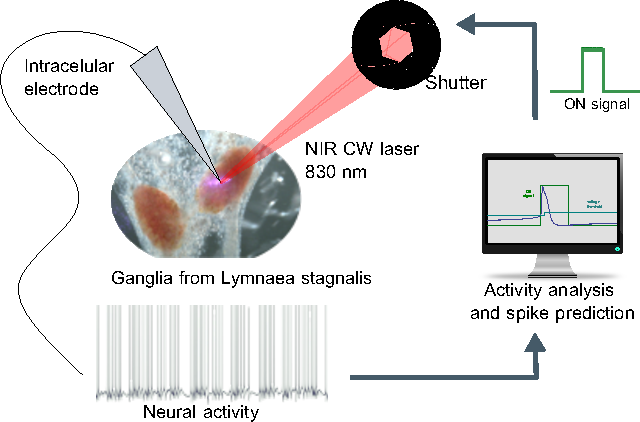
\includegraphics[width=\textwidth]{img/laser/activity_dependent_protocol.pdf}
	\caption{Activity-dependent protocol scheme. Neurons were recorded intracellularly and their voltage signals were processed in real-time with the RTXI software. Using the spike prediction algorithms, the shutter was triggered at the desired action potential phase illuminating the neurons.}
	\label{fig:activity dependent protocol}
\end{figure}


The main challenge in this protocol is the identification of the specific phase of the spike waveform to deliver the stimulus, i.e., predicting the spike, since spontaneous neural activity has intrinsic variability that requires the online adaptation of specific thresholds instead of a hand-tuned preset value. For this purpose, the protocol relied on the reference values from the previous spike at a specific time interval from the peak. The voltage threshold was calculated based on the voltage value measured in the previous spike, and recalculated at each action potential. Thus, after each spike, the threshold for the spike prediction was updated using the following equation:

\begin{equation}
	\centering 
	V_{threshold}=V[t_{spike}[i-1]-\tau],
\end{equation}

\noindent with $\tau$ being the selected time for the prediction before the spike and $t_{spike}$ the time instant of the spike peak.

This prediction is effective for stereotyped spikes when only low amplitude subthreshold oscillations occur, but it is limited in other scenarios. Therefore, for neurons or action modes of the same neuron when it was necessary to stimulate before the depolarization rise, another reference was used: the area of the recorded voltage. In this other mode of the protocol defined in Eq. \ref{eq:area}, the voltage was accumulated along the activity and the sum was reset after each spike. 

\begin{equation}
	\centering 
	V_{area}=\int_{V[spike_{i-1}]}^{V[spike_{i}]}V(t).
	\label{eq:area}
\end{equation}

The stimulation was triggered when the area reached a specific threshold, which was predicted as in the voltage case, or hand-tuned. For the detection of the minimum point to reset the voltage area, we used a RTXI module based on RTHybrid, a real-time software that includes automatic adaptation algorithms to handle the ongoing variability of the recordings \parencite{amaducci_rthybrid_2019,reyes-sanchez_automatic_2020,reyes-sanchez_automatized_2023}, \href{https://github.com/GNB-UAM/rthybrid-for-rtxi/tree/master/rthybrid_burst_analysis}{github.com/GNB-UAM/RTHybrid-For-RTXI}. The use of each mode of the protocol in the experiment was decided depending on the specific requirements of the recorded activity. 

\begin{figure}[htb!]
	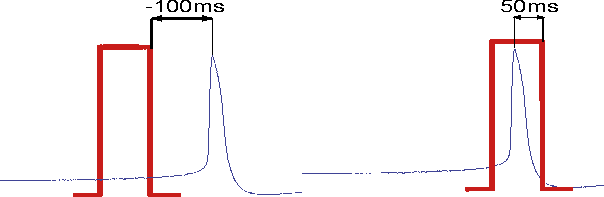
\includegraphics[width=\textwidth]{img/laser/offset_examples.pdf}
	\caption{Examples of illumination offset, defined as the time interval from the end of the illumination to the peak of the spike.}
	\label{fig:offset_example}
\end{figure}

Using this detection protocol, we assessed the effect of the illumination at different phases of the action potential in the range from 100 ms before the spike peak to 80 ms after the spike peak (see an example of the illumination offset in Fig. \ref{fig:offset_example}). The illumination interval was 58 ms, validated as the minimal duration for effective stimulation in the test trials. The RTXI module programmed for this study is available at \href{https://github.com/GNB-UAM/spike_predictor}{github.com/GNB-UAM/spike\_predictor}.

\subsection{Spike waveform characterization parameters} \label{sec:characterization parameters}
\label{sect:metrics}
For both experimental recordings and model simulations, action potentials were detected as the maximum point over a threshold, and each waveform was segmented 100ms before and after the peak temporal reference. For the superposition of action potentials (Figs. \ref{fig:continuous_results_panel},\ref{fig:continuous_model},\ref{fig:temperature model}) the waveforms were aligned in the $x$-axis by the peak and in the $y$-axis by the first point of the waveform voltage values.

\begin{figure}[htb!]
	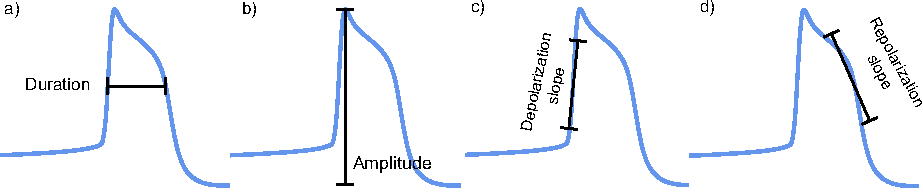
\includegraphics[width=\textwidth]{img/laser/spike_metrics.pdf}
	\caption{Representation of waveform shape's metrics: a) Spike duration at half width. b) Spike amplitude between the maximum and minimum voltage values. c) Depolarization slope at half width. d) Repolarization slope at half width.}
	\label{fig:spike metrics}
\end{figure}


For the waveform shape characterization, we used four metrics: duration, amplitude, depolarization and repolarization slopes. They are depicted in Fig. \ref{fig:spike metrics} and defined as follows:
\begin{itemize}
	\item Duration: Time interval between the two points at half width of the action potential. 
	\item Amplitude: Difference between minimum and maximum voltage values in the waveform in the analyzed segment. 
	\item Depolarization slope: Slope in the depolarization phase (previous to the peak) measured 1 ms before and after the half width point reference.
	\item Repolarization slope: Slope in the repolarization phase (after the peak) measured 1 ms before and after the half width point reference.
\end{itemize}

These metrics were used for the quantitative analysis of the change in experimental recordings and model simulations. In Sec. \ref{sect:statistical_analysis} below we describe the quantification methodology for the waveform metric change as well as for the comparison between the experimental and model results.



\subsection{Statistical Analysis}
\label{sect:statistical_analysis}
The statistical significance analysis in the data obtained from the sustained CW-NIR stimulation protocol in Figure \ref{fig:continuous_results_panel} was performed applying a paired T-test to the four spike waveform metrics characterized here (see Fig. \ref{fig:spike metrics} Data from distinct experiments was gathered and paired by recordings of control-laser and control-recovery (see Fig. \ref{fig:continuous_results_panel}C). The null-hypothesis tested was that control group was equal to the laser group and that the control group was equal to the recovery group, respectively. Since we performed the test in the four waveform metrics --spike duration, depolarization slope, repolarization slope and amplitude-- we applied the Bonferroni correction, thus we considered high-significance when $\rho < 0.01/4$.

To compare recordings from different neurons, we normalized the change between the laser and the control conditions for each waveform metric using the following expressions for electrophysiological data:

\begin{equation}
	{metric\ change}_{experimental} = \frac{|\mu(metric_{laser}) - \mu(metric_{control})|}{|\mu(metric_{control})|},
\end{equation}
\noindent where $\mu(metric_{laser/control})$ is the mean of the corresponding metric for all waveforms in a given laser stimulation or control trial.

Analogously, to compare the change between the distinct model simulations we normalized the change in the parameter-driven simulated variability range using the following expression:

\begin{equation}
	\label{eq: model change}
	{metric\ change}_{model} = \frac{|metric_{min} - metric_{max}|}{|metric_{max}|},
\end{equation}

\noindent where $metric_{min/max}$ refers to the minimum or maximum value of the corresponding waveform metric resulting from the model simulations in the  considered parameter range.


For the comparison between experimental data and model simulations in Figure \ref{fig:continuous_model}, we defined an experimental reference for each metric as the general mean and standard deviation for all experiments ($N=23$). This allowed us to define a range of change due to the laser effect to which the model values could be compared. The mean of metric experimental change (MEC) was defined as:
\begin{equation}
	\mu_{MEC} = \frac{1}{N}\sum_{i=1}^{N}\frac{|\mu(\text{metric})_{\text{laser}} - \mu(\text{metric})_{\text{control}}|_{i}}{|\mu(\text{metric})_{\text{control}}|_{i}},
\end{equation}

Here, $\mu(\text{metric})_{\text{laser}}$ and $\mu(\text{metric})_{\text{control}}$ represent the mean values for each experiment $i$ in laser stimulation and control trials, respectively, where the index $i$ ranges for all experiments, with $N$ being the number of experiments.

Thus, the percentage change in waveform from the model simulations, as described in equation \ref{eq: model change}, was mapped to this reference range: $(\mu_{MEC}\pm2\sigma_{MEC})$, with $\sigma_{MEC}$ being the standard deviation of the MEC. To visually represent this range, we utilized a color gradient with the \textit{background\_gradient} option in \textit{DataFrame} style in Python. The formula for mapping these values is:

\[\text{Gradient value} = \frac{\text{value} - \text{Vmin}}{\text{Vmax} - \text{Vmin}}\]

Here, \textit{value} represents the percentage change in the model simulation for a specific metric, while \textit{Vmin} and \textit{Vmax} represent $\mu_{MEC}-2\sigma_{MEC}$ and $\mu_{MEC}+2\sigma_{MEC}$ respectively, with $\mu_{MEC}$ and $\sigma_{MEC}$ being the specific mean and standard deviation corresponding to the metric specified in \textit{value}. Since all changes are in absolute value, the lower bound for Vmin is 0.

All data analyses were performed in Python, the scripts are available in \href{https://github.com/GNB-UAM/Garrido-Pena_Modulation-neural-dynamics-by-CW-NIR-stimulation}{github.com/GNB-UAM/Garrido-Pena\_Modulation-neural-dynamics-by-CW-NIR-stimulation}.
